\subsection{Random Forests}

A random forest was computed in figure \ref{fig:success_time_vs_trees_randomForest} using G3M2 data as test set and the remaining 14 students as train set.
The number of trees was varied and the time measured.

\begin{figure}[H]
\centering
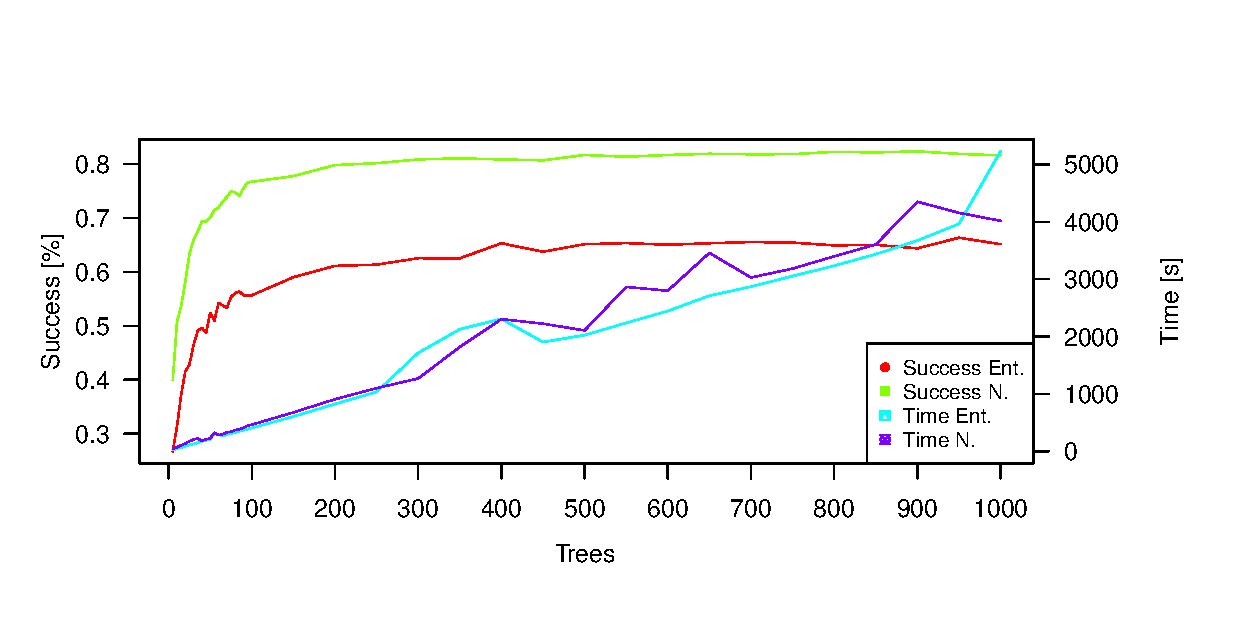
\includegraphics[width = 0.95 \textwidth]{graphics/successRate_randomForest}
\caption{Success rate and time taken to compute the trees needed in the random forest as the number of trees increases.}
\label{fig:success_time_vs_trees_randomForest}
\end{figure}

As can be seen on figure \ref{fig:success_time_vs_trees_randomForest}, then the success rate increases drastically from 0 to 100 trees in the random forest and it settles around 64\% and 80\% for the entropy and z-score normalized data respectively.
The time increases linearly with the number of trees, but with some inconsistencies, probably because of the computer scheduler taking time of for other tasks.

From figure \ref{fig:success_time_vs_trees_randomForest} it was decided to use 200 trees for the optimum random forest for both methods.
Figure \ref{fig:success_randomForest} was generated using the 200 trees.
Each point was computed using a single person in the test set and independently the 14 other in the training set.

% e 0.37425 0.4405 0.34075 0.52500 0.42350 0.4395 0.45675 0.60175 0.63925 0.44125 0.44650 0.539 0.5560 0.49575 0.28800
% n 0.36400 0.6030 0.45450 0.64275 0.60675 0.6170 0.63025 0.79775 0.71775 0.63600 0.65225 0.762 0.6795 0.55875 0.41125
% "mean e: 0.467183333333333"
% "mean n: 0.6089"
\begin{figure}[H]
\centering
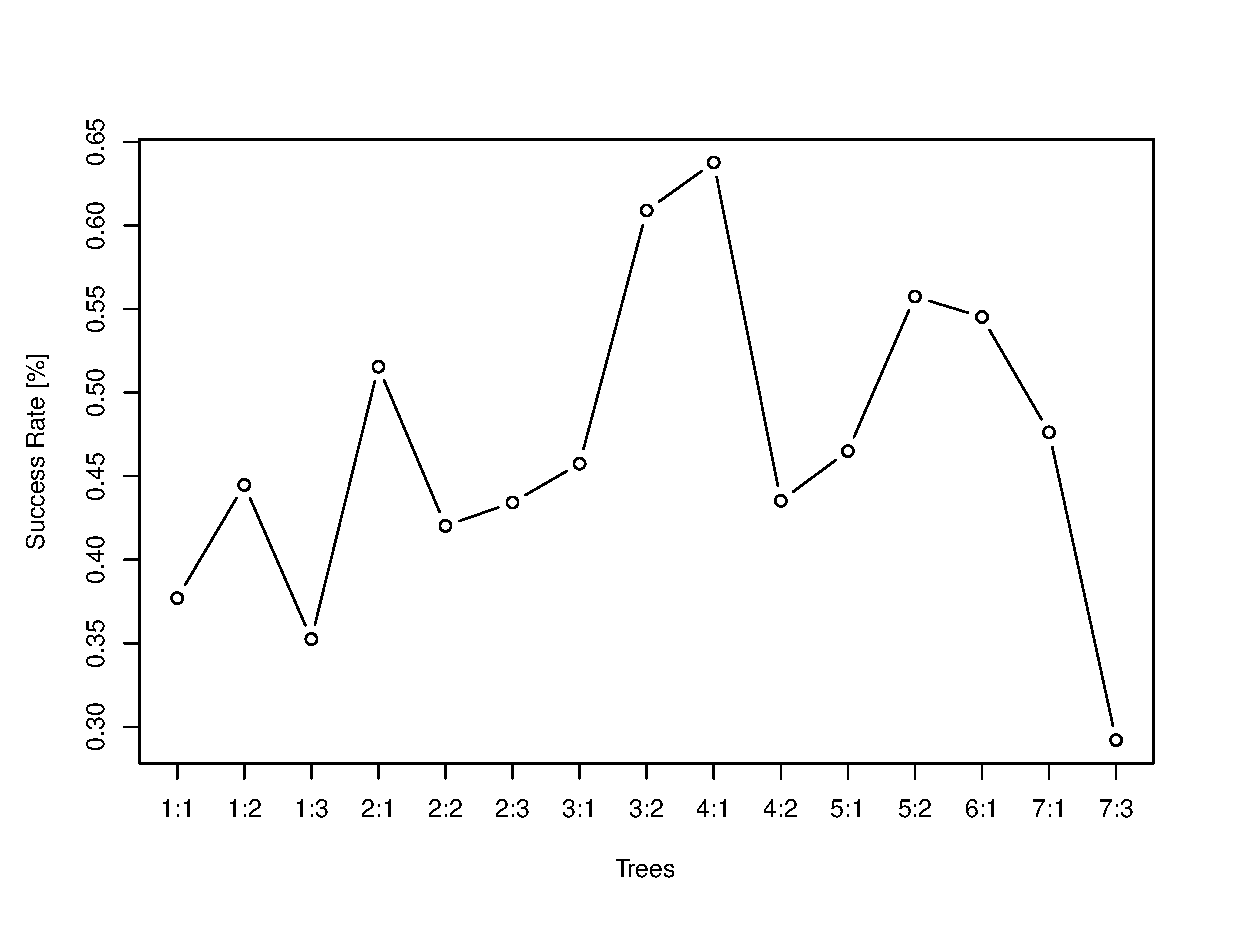
\includegraphics[width = 0.95 \textwidth]{graphics/successRate_randomForest_comp}
\caption{Success rate for the different people given they are not present in the data set. The mean success rate is 46.7\% for the entropy normalized dataset and 60.9\% for the z-score normalized.}
\label{fig:success_randomForest}
\end{figure}